% Figure 13 -- Seiberg-Witten graphs for (A3,A2), (A3,A3), (A3,A4)
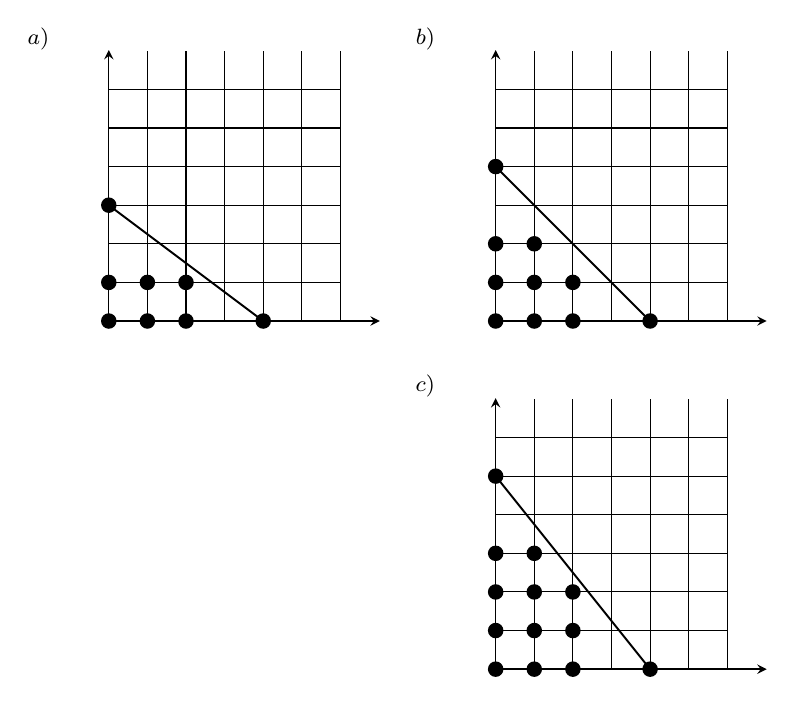
\begin{tikzpicture}[x=1pt,y=1pt,>=stealth,line width=0.5pt]
  \def\u{13.95}
  % ================= panel a) =================
  \begin{scope}[xshift=48.3pt,yshift=134.5pt]
    \draw[line width=0.4pt] \foreach \i in {1,...,6} {(\i*\u,0) -- (\i*\u,{7*\u})};
    \draw[line width=0.4pt] \foreach \j in {1,...,6} {(0,\j*\u) -- ({6*\u},\j*\u)};
    \draw[->] (0,0) -- (0,{7.02*\u});
    \draw[->] (0,0) -- ({7.02*\u},0);
    \draw[line width=0.7pt] (0,{3*\u}) -- ({4*\u},0);
    \foreach \i/\j in {0/0,1/0,2/0,4/0,0/1,1/1,2/1,0/3}
      {\fill ({\i*\u},{\j*\u}) circle[radius=2.8pt];}
  \end{scope}
  % ================= panel b) =================
  \begin{scope}[xshift=188.1pt,yshift=134.5pt]
    \draw[line width=0.4pt] \foreach \i in {1,...,6} {(\i*\u,0) -- (\i*\u,{7*\u})};
    \draw[line width=0.4pt] \foreach \j in {1,...,6} {(0,\j*\u) -- ({6*\u},\j*\u)};
    \draw[->] (0,0) -- (0,{7.02*\u});
    \draw[->] (0,0) -- ({7.02*\u},0);
    \draw[line width=0.7pt] (0,{4*\u}) -- ({4*\u},0);
    \foreach \i/\j in {0/0,1/0,2/0,4/0,0/1,1/1,2/1,0/2,1/2,0/4}
      {\fill ({\i*\u},{\j*\u}) circle[radius=2.8pt];}
  \end{scope}
  % ================= panel c) =================
  \begin{scope}[xshift=188.1pt,yshift=8.7pt]
    \draw[line width=0.4pt] \foreach \i in {1,...,6} {(\i*\u,0) -- (\i*\u,{7*\u})};
    \draw[line width=0.4pt] \foreach \j in {1,...,6} {(0,\j*\u) -- ({6*\u},\j*\u)};
    \draw[->] (0,0) -- (0,{7.02*\u});
    \draw[->] (0,0) -- ({7.02*\u},0);
    \draw[line width=0.7pt] (0,{5*\u}) -- ({4*\u},0);
    \foreach \i/\j in {0/0,1/0,2/0,4/0,0/1,1/1,2/1,0/2,1/2,2/2,0/3,1/3,0/5}
      {\fill ({\i*\u},{\j*\u}) circle[radius=2.8pt];}
  \end{scope}
  % ================= panel labels =================
  \node[inner sep=0pt] at (22.9,236.5) {\fontsize{8}{10}\selectfont$a)$};
  \node[inner sep=0pt] at (162.7,236.5) {\fontsize{8}{10}\selectfont$b)$};
  \node[inner sep=0pt] at (162.7,111.1) {\fontsize{8}{10}\selectfont$c)$};
\end{tikzpicture}
